\chapter{Solicitar OS - Integração com o SEI - Solicitação}

\section{Detalhamento do cenário ``Incluir Solicitação''}

Na EPE: \textbf{``Solicitar Ordem de Serviço''}

Na funcionalidade: \textbf{``02 - Incluir Solicitação''}

\begin{nota}[1]{02 - Incluir Solicitação}
	Quando o usuário solicita "Enviar para Assinatura"
	
	Então o sistema realiza solicitação em nome da unidade selecionada pelo o Usuário
	
	E gera um processo no SEI
	
	E gera um arquivo html padrão da solicitação para ser assinado no SEI
	
	E envia os anexos
	
	E gera bloco de assinatura no SEI
	
	E torna o status da solicitação como: "Enviado para assinatura"
	
	E apresenta a mensagem: "Enviado com sucesso!"
\end{nota}


	\begin{quotation}
		\Large
		Detalha-se, a seguir, a sequência de ações que o Sistema ASSEL deve realizar após o clique no botão ``Enviar para Assinatura''.
		\normalsize
	\end{quotation}


	\begin{figure}[htbp!]
	\centering
	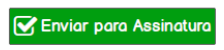
\includegraphics[width=0.5\textwidth]{fig/solicitaros-sei/botaoenviarparaassinatura.png}
	\end{figure}	

\newpage

\Large
\begin{center}
	\textbf{INÍCIO}
\end{center}
\normalsize

\subsection{Sistema ASSEL cria novo processo no SEI}	
	
	Um novo processo do tipo \textbf{``Assessoria Legislativa: Consulta, estudo, parecer, discurso e proposições legislativas''} deve ser automaticamente criado no SEI pelo Sistema ASSEL. 
	
	\begin{itemize}
		\item Esse processo deve ser criado na Unidade do SEI do Solicitante. 
		
		\item O processo deve possuir o Nível de Acesso especificado pelo Solicitante na Funcionalidade ``Incluir''. Caso o Nível escolhido foi ``Restrito'', deve-se 
		utilizar a ``Hipótese Legal'' escolhida na mesma tela da funcionalidade.
		
		\item O número do processo do SEI recém criado deve ser armazenado como atributo da Solicitação no sistema ASSEL  de forma que conste na sub-funcionalidade ``Visualizar'' da funcionalidade ``Solicitar Ordem de Serviço''.  
	\end{itemize}


	\begin{exemplo}[1]{Exemplo}
		Sistema ASSEL cria o processo número 00001-00000001/2021-01.
	\end{exemplo}
	
	
\subsection{Sistema ASSEL cria documento da OS no processo do SEI}

	Deve ser criado um primeiro documento no Processo do tipo \textbf{``SOLICITAÇÃO DE SERVIÇO DA ASSESSORIA LEGISLATIVA''} já preenchido com as informações fornecidas pelo Solicitante no Sistema ASSEL. Este é o documento que deverá ser assinado.
	
	
	\begin{itemize}
		\item O número do documento do SEI relacionado à Ordem de Serviço que deverá ser assinado deve ser armazenado como atributo da Solicitação no sistema ASSEL  de forma que conste na sub-funcionalidade ``Visualizar'' da funcionalidade ``Solicitar Ordem de Serviço''. 
	\end{itemize}

	\begin{exemplo}[1]{Exemplo}
		Sistema ASSEL cria o documento Número 0000001 no processo 00001-00000001/2021-01.
	\end{exemplo}

\subsection{Sistema ASSEL insere os anexos no processo}
		
	No processo, logo abaixo desse documento com a OS que será assinada, deverão ser automaticamente inseridos os anexos fornecidos pelo solicitante ao Sistema ASSEL \emph{respeitando os Níveis de Acesso e Hipóteses Legais escolhidas pelo usuário}. 
		
\subsection{Sistema ASSEL cria, caso necessário, o Bloco de Assinatura}	
	

\subsubsection{Caso o Usuário Solicitante Pertença à Unidade Solicitante do SEI}

	Se a Unidade Solicitante possui o Usuário que está fazendo a Solicitação como um usuário pertencente a ela\footnote{Isso deve ser verificado usando a API do SEI}, não precisa criar Bloco de Assinatura. E nem seria possível fazer isso. 
	
	Nesse caso, sistema deve avisar ao Usuário para assinar o documento especifico do processo especifico da unidade determinada conforme exemplo de mensagem abaixo:
	

	\begin{exemplo}[1]{Exemplo de Mensagem em Caso de Não Haver Bloco de Assinatura}
		Por favor, assinar o documento SEI Nº 0000001 do processo 00001-00000001/2021-01 na Unidade ``NOME DA UNIDADE'' para concluir a solicitação. 
			
		\vphantom{espaço vertical em branco}			
					
		Após assinatura, o Sistema ASSEL se encarregará de tramitar o processo para a Assessoria Legislativa.
		
		\vphantom{espaço vertical em branco}					

		\framebox[3cm][c]{OK}
	\end{exemplo}
	
	
	
\subsubsection{Caso o Usuário Solicitante NÃO Pertença à Unidade Solicitante do SEI}
	
	
	\begin{enumerate}

	
	\item  Se a Unidade Solicitante não possui o Usuário que está fazendo a Solicitação, então será mostrado uma janela \textbf{Popup} contendo um \emph{combobox} listando todas as unidades (exceto a Unidade Solicitante\footnote{Lembrar  que na lista de unidades do combobox não deve constar a Unidade do SEI onde está sendo criado o Bloco de Assinatura já que não é possível criar um Bloco de Assinatura e disponibiliza-lo para a mesma unidade de origem.}) de forma que o Usuário possa escolher para qual Unidade do SEI deverá ser disponibilizado o Bloco de Assinatura que será assinado.

	\begin{env-popup}[1]{Exemplo de Popup}
	Por favor, escolha a unidade do SEI onde você deseja assinar a solicitação:
	
	\vphantom{espaço vertical em branco}			
	
	\framebox[8cm][c]{CMI}		
	\framebox[0.5cm][c]{$\nabla$}
	
	\vphantom{espaço vertical em branco}					
	
	
	\framebox[3cm][c]{OK}
	\framebox[3cm][c]{CANCELAR}
	
	\end{env-popup}	

	\item Quando o usuário escolhe uma Unidade do SEI e clica em OK, o sistema verifica se o Usuário tem acesso no SEI àquela unidade \emph{e se possui capacidade de assinar documentos nela}. Se sim, prossegue. Se não, pede que ele escolha uma Unidade onde ele tem acesso e pode assinar. Só prossegue quando o Usuário escolher uma unidade que atenda esses dois requisitos. 	


	\item Quando finalmente o usuário escolhe uma unidade na qual ele tem acesso e tem permissão de assinar documentos, então o sistema cria o bloco de assinatura na Unidade Solicitante.
	
	\item O Bloco de Assinatura deve ser criado com a seguinte ``Descrição'' padrão:
	
	\begin{exemplo}[1]{Descrição do Bloco de Assinatura}
		Sistema ASSEL - Solicitação de Serviço

		Unidade Solicitante: Gabinete do Deputado Fulano

		Usuário Solicitante: Nome Completo do Usuário Solicitante
	\end{exemplo}
	
	
    %\begin{figure}[htbp!]
	%\centering
	%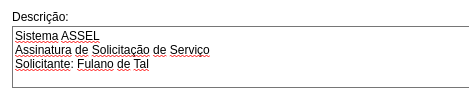
\includegraphics[width=0.8\textwidth]{fig/solicitaros-sei/ex2.png}
	%\caption{Exemplo de Descrição do Bloco de Assinatura}
	%\label{fig:solitaros-sei:ex2}
	%\end{figure}	
	
	\item No campo ``Unidades para Disponibilização'' deve ser escolhido a unidade escolhida pelo Usuário Solicitante no \textbf{Popup}.

    \begin{figure}[htbp!]
	\centering
	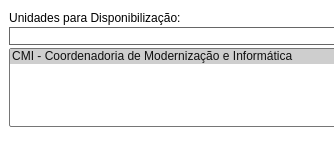
\includegraphics[width=0.8\textwidth]{fig/solicitaros-sei/ex3.png}
	\caption{Exemplo de Unidade para Disponibilização do Bloco de Assinatura}
	\label{fig:solitaros-sei:ex3}
	\end{figure}


	\item Em seguida, o sistema cria o Bloco de Assinatura dentro da Unidade Solicitante (onde o processo foi criado) e incluí nele o documento do processo relativo à OS que precisa ser assinada. Finalmente, o sistema disponibiliza o Bloco de Assinatura para ser assinado pelo Usuário Solicitante.

	\item O número do bloco de assinatura deve ser armazenado como atributo da Solicitação no sistema ASSEL de forma que conste na sub-funcionalidade ``Visualizar'' da funcionalidade ``Solicitar Ordem de Serviço''. 

	\item De forma semelhante, o Sistema ASSEL mostra a mensagem ao usuário informando que ele deve assinar o documento no Bloco de Assinatura criado.
	
	
	\begin{exemplo}[1]{Exemplo de Mensagem em Caso de Haver Bloco de Assinatura}
	Por favor, assinar o documento SEI Nº 0000001 do processo 00001-00000001/2021-01 disponível no Bloco de Assinatura Nº 00001 disponibilizado para a Unidade UNIDADE-ESCOLHIDA. 
	
	\vphantom{espaço vertical em branco}			
	
	Após assinatura, o Sistema ASSEL se encarregará de tramitar o processo para a Assessoria Legislativa.

	\vphantom{espaço vertical em branco}	
					
	\framebox[3cm][c]{OK}
\end{exemplo}	
	
	
	\end{enumerate}	
	


\subsection{Sistema ASSEL aguarda assinatura do Usuário Solicitante}

A partir daí o sistema passa a monitorar o documento do SEI esperando que ele seja assinado.
	
\subsection{Usuário Assina}

Usuário acessa o SEI e assina o documento.


\subsection{Sistema ASSEL cancela e conclui Bloco de Assinatura caso ele exista}

Após assinatura, se foi criado Bloco de Assinatura, o Sistema cancela a disponibilização do Bloco de Assinatura para as unidades e o conclui.

\subsection{Sistema Envia Processo para a Unidade ASSEL}

O Sistema envia o processo para a Unidade ``ASSEL''.

\subsection{Sistema Recebe o Processo na Unidade ASSEL}

Do lado da ASSEL, o próprio sistema recebe o processo.

\subsection{Sistema atribui ao processo um Acompanhamento Especial}

Sistema marca o processo com o Acompanhamento Especial especificado.

\subsection{Sistema conclui o processo}

Sistema conclui o processo para remove-lo da lista de ``Recebidos'' do SEI da Unidade ASSEL.

\Large
\begin{center}
	\textbf{FIM}
\end{center}
\normalsize


\section{Atualização}

	Na reunião do dia 01/12/21 com Daniel e Gustavo ficou definido 	que o Sistema ASSEL ia monitorar as assinaturas de documentos a cada meia hora por 15 dias. Caso esses documentos não fossem assinados nesse prazo, eles seriam automaticamente cancelados.


